\chapter{Results}
\label{chap:results}
%Link to audio examples (ok)
In this chapter, I compare the results of the experiments listed in Section \ref{sec:experiments-autotune}. I then describe the design and responses for a subjective listening test on the outputs of the most successful experiment. In the subjective test, I compare the outputs of the proposed system to the original singing and to a baseline system that shifts the pitch to the nearest equal-tempered scale frequency. Audio examples are publicly available\footnote{\href{https://adding-this-link}}.

%Synthesized set
\section{Experiments on the synthesized test set}
Table \ref{table:experiment-results} shows the validation and test MSE losses for all experimental configurations. For readability, the MSE is converted to cents. MSE loss was computed based on synthesized data, where in-tune performances were de-tuned, making it possible to have an objective error metric. We note that the error is not based on the audio outputs but on the pitch shifts. However, audio examples online enable the reader to hear the effects of the system. We see that ... Our MSE was reduced ...  How does an average error of ... cents translate to good intonation? The average error includes the notes where the prediction was relatively close to the target and those where the prediction shifted the pitch in the opposite direction. For this reason, the mean error only provides a general idea of overall accuracy. When musicians fine-tune their intonation, shifts are often in the range of 5 cents---for a fifth---to 16 cents---for a third. If the mean error falls into this general area, it indicates that the adjustments predicted by the system fall into the same order of magnitude at least some of the time. 

From the fact that the model converged to a reasonably small error, we can conclude that the proposed model works on unseen signals if the detuning behavior is similar to that of the synthetic training signals. In the next section, we test our model on real-world singing signals.

%- MSE before and after for training, validation, test
\begin{table*}
\centering.
\begin{tabular}{ |c|c|c|c| } 
\hline
\multicolumn{4}{|c|}{\textbf{Experiments: MSE after training}}\\
\hline\hline
\textbf{Model names} & Validation loss & Test loss & Steps trained \\
\hline\hline
Note-runif-1e-5 & 0 & 0 & 0  \\
\hline
Note-runif-5e-6 & 0 & 0 & 0  \\
\hline
Note-HMM-1e-5 & 0 & 0 & 0  \\ 
\hline
Song-runif-1e-5 & 0 & 0 & 0  \\ 
\hline
Song-runif-5e-6 & 0 & 0 & 0  \\ 
\hline
Song-HMM-1e-5 & 0 & 0 & 0  \\ 
\hline
Song-HMM-5e-6 & 0 & 0 & 0  \\ 
\hline
Song-HMM-pretrain-1e-5 & 0 & 0 & 0  \\ 
\hline
Song-runif-pretrain-1e-5 & 0 & 0 & 0  \\
\hline
\end{tabular}
\label{table:experiment-results}
\caption{Validation and test losses in cents after convergence for the experiment configurations listed in Section \ref{sec:experiments-autotune}. Loss is computed on synthesized samples, where in-tune performances were de-tuned, making it possible to compute an objective error metric. We see that ... performed best ...}
\end{table*}
%- Loss curves
%- Analysis
%Subjective listening test
\section{Subjective listening test}
\label{sec:subjective-test}
%- Listening test setup
Given that we do not have ground-truth shifts for real-world performances, we can evaluate the proposed model's performance using a subjective listening test. Listeners compared excerpts from the original performances to those pitch-shifted using the proposed system. They also compared both versions to the output of a baseline pitch correction system. 

The baseline model is inspired by the Antares Auto-Tune system, but shifts pitch the same way as the proposed system for a fair comparison. The baseline shifts each note so that its median is around the nearest equal-tempered scale frequency. The note is shifted by a constant, unlike Auto-Tune, which shifts every frame to the nearest frequency while applying adjustments based on the \textit{retune speed}, \textit{humanize}, and other parameters. Given that it always finds the nearest frequency, the program can only apply shifts of up to 50 cents. 

All shifts applied to the audio were computed using TD-PSOLA. The only difference between the outputs is the amount of shift. In a small-scale subjective test conducted in \cite{wager2020deep}, listeners were asked to select which version sounded more natural. Listeners did not hear a difference between samples, which indicates that TD-PSOLA doesn't produce a significant amount of artifacts that would make it difficult to rate the quality of the system only based on musical intonation instead of audio quality.

\subsection{Subjective test design}
The first decision to make for the subjective test was how long excerpts to use. In subjective tests for audio quality such as MUSHRA \cite{mushra}, samples tend to be short---around 10 seconds---because our auditory memory fades quickly. The longer the excerpt, the harder it is to compare the quality with confidence. Longer excerpts also result in more ambiguity, as some parts of the signal might sound better in one version at the beginning, and in another version at the end. These challenges apply to musical intonation. What if a singing excerpt shifted by the proposed system sounded excellent for all notes but one, and completely wrong for the remaining note, whereas the excerpt it was compared to would sound slightly off for most notes, but never far off? This ambiguity provides a reason to keep clips short. However, they cannot be too short, or the listener won't have the chance to hear the harmonic and melodic context. I finally decided, based on listening to many examples, to choose 12 seconds, where the first and last second are used for fading in and out, so are only partially audible. I also structured the test interface so that the listeners could play the samples as much as they wished and could restrict the playback to a smaller window to focus on details. %We also asked them to select the version they found more natural, but received the feedback that users heard no difference, confirming that our TD-PSOLA implementation usually produced clean results.

I randomly sampled 4 12-second clips from each of the ... test performances---original, pitch shifted using the proposed system, and pitch shifted using the baseline---controlling for vocals presence in 70\% of the frames. I lowered this threshold if four such clips could not be found. The process resulted in ...  performance clips with 3 versions per clip. 

I structured the test as a blind paired comparison test. Each listener was randomly assigned ... comparisons per test but could take the test more than once. For each clip, the listener was randomly assigned 2 out of the 3 versions for comparison. For example, a listener might compare the baseline output of a clip to the original performance clip, or the baseline to the proposed system. 

\begin{figure}[t]
    \centering
    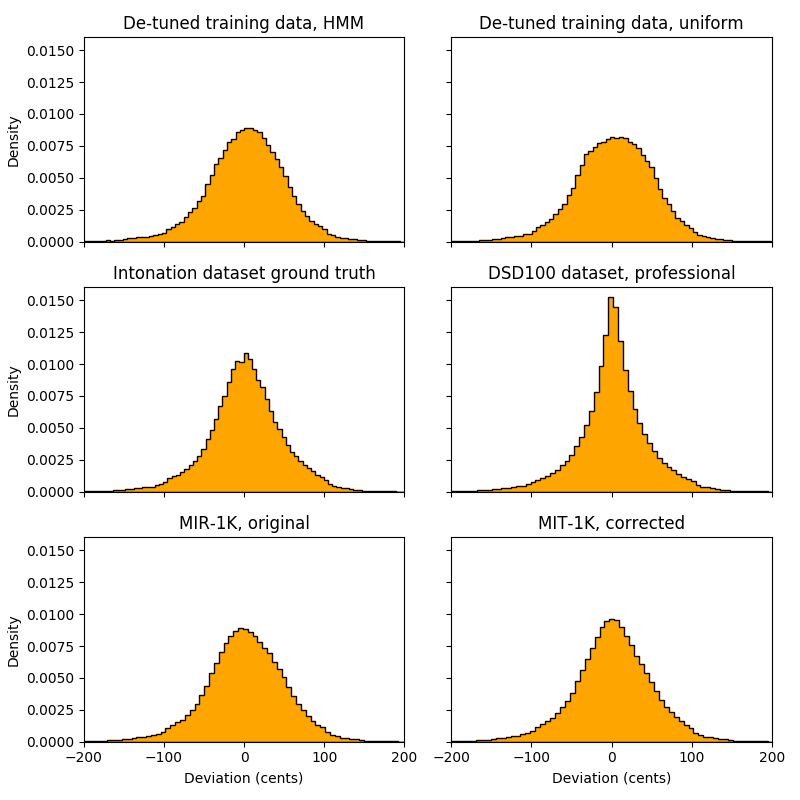
\includegraphics[width=\columnwidth]{figures/dataset-comparison.png}
    \caption{Subjective listening test interface. We note the slider at the bottom that enables the listener to restrict the playback range.}
    \label{fig:listening-test-ide}
\end{figure}

\begin{figure}[t]
    \centering
    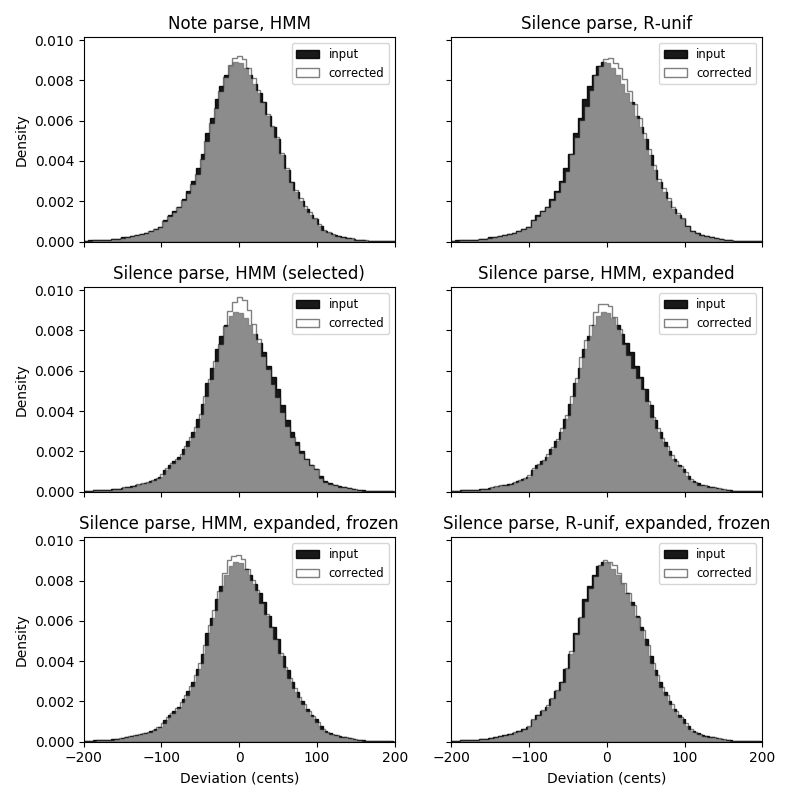
\includegraphics[width=\columnwidth]{figures/mir-1k-comparison.png}
    \caption{Subjective listening test interface. We note the slider at the bottom that enables the listener to restrict the playback range.}
    \label{fig:listening-test-ide}
\end{figure}

\begin{figure}[t]
    \centering
    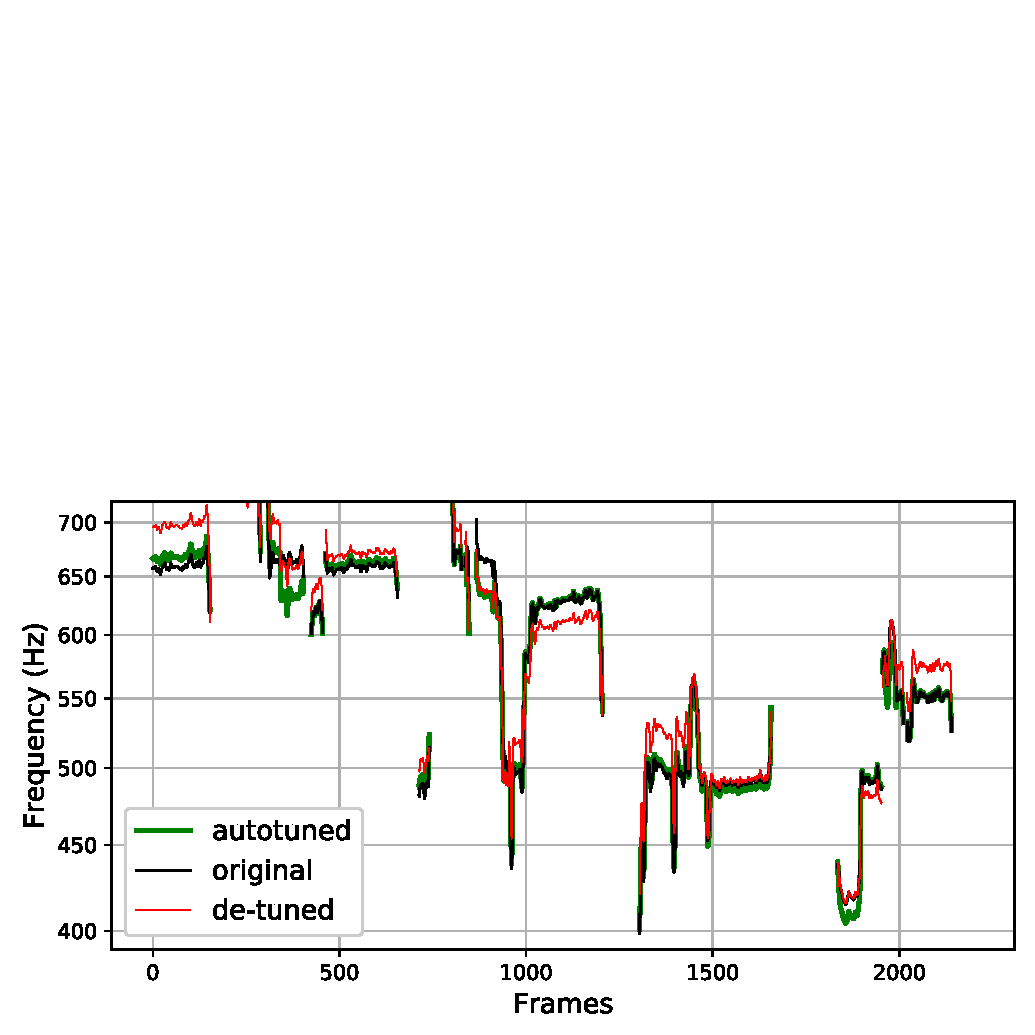
\includegraphics[width=\columnwidth]{figures/results.pdf}
    \caption{Subjective listening test interface. We note the slider at the bottom that enables the listener to restrict the playback range.}
    \label{fig:listening-test-ide}
\end{figure}

The test interface---shown in Figure \ref{fig:listening-test-ide}---prompted people to select the version they found more accurate, referring to harmonic alignment between the singing voice and the backing track. At the beginning of the test, I included YouTube links to the original performances of each featured song so that listeners not familiar with the music could get to know the melody and chord progression. I also provided two practice examples to listen to in advance. The test was voluntary and anonymous. Listeners were not aware of the three different cases being compared, only that they were evaluating comparative pitch quality. 

10 different subjects with formal musical training provided a total of 138 responses. 

The test included a ``quiz'' question to make sure that responses for each test were valid. In this question, the original was paired with a version where every note was shifted by a random amount up to 100 cents, and manually selected to sound noticeably out of tune. All participants answered correctly, which may be due to the fact that they were all musically trained. A musically untrained person who gave feedback on the test did not answer the question correctly.

%- Results
\subsection{Results on the subjective listening test}
\label{sec:subjective-results}
Globally, in pairs where the subjects compared the proposed program to the original performance, they selected the proposed 33 times and the original 35 times, for a success rate of 49\% with a one-sided binomial test p-value of 0.45. The baseline versus the original produced numbers 24 and 34, or 41\% success rate with p-value 0.12. The proposed model versus the baseline produced 31 and 29, or a success rate of 52\% with p-value 0.45. These global numbers themselves do not suggest an advantage in using either pitch corrector. The number of responses is also quite small, which leaves uncertainty in these responses because not all versions of all 96 clips were covered and each clip is quite different. In future work, we plan to conduct a larger-scale subjective test.

In our small sample, we found some patterns worth investigating once we conduct a larger test. One such pattern is that subjects might prefer proposed corrected signals when the quality of the original singing is slightly off key, but not too far. We identify such cases by looking at note-level pitch deviation statistics (in cents) between the original performance and the ground-truth MIDI score, generously provided by Smule, Inc. For example, we computed the standard deviation of the cents differences between the original singing and the ground-truth MIDI score. We found that the subjects usually favor a corrected example if the original was within a particular standard deviation range (between 40 and 60 cents). 19 out of 24, or 79\% of the preferred corrected examples were in this range, compared to only 16\% (3 out of 19) preferred original examples. While we would need more data for reliable results, we expect this behavior due to the imperfectly tuned nature of our crowdsourced training data used as in-tune ground truth---only some noticeable amount of off-pitch can be fixed by the trained model. Meanwhile, the model is exposed only to up to a semitone pitch shift, suggesting that too much variation in the test signal cannot be fixed, either. 

We also compared the proposed method to the baseline. In 18 out of 21 or 86\% of performances where the proposed model was selected, the median of the absolute value of deviations in cents within two semitones was less than 46. However, 8 out of 20, or 40\% of performances where the baseline was selected were in the same range. This second result again that the proposed model might work better when performances are already relatively accurate. See Table \ref{tab:result-autotune} for a summary. 

\begin{table}[t]
  \begin{center}
  \vspace{-0.05in}
    \caption{The subjective test results that contrast different distributions of the corrected, baseline, and original examples. Section \ref{sec:subjective-results} describes the ranges in question.}
    \begin{tabular}{|l||c|c|}
    \hline
      & Within range & Out of range \\
      \hline
      Preferred corrected examples & 79\% & 21\% \\
      Preferred original examples & 16\% & 84\% \\
      \hline
      Preferred corrected examples & 87\% & 13\% \\
      Preferred baseline examples & 22\% & 78\% \\
      \hline
    \end{tabular}
    \vspace{-0.2in}
    \label{tab:result-autotune}
  \end{center}
\end{table}
%- Analysis

